%%%%%%%%%%%%%%%%%%%%%%%%%%%%%%%%%%%%%%%%%
% Oliver Lemon made minor edits (jan 2015)  to : 
% Masters/Doctoral Thesis 
% LaTeX Template
% Version 1.43 (17/5/14)
%
% This template has been downloaded from:
% http://www.LaTeXTemplates.com
%
% Original authors:
% Steven Gunn 
% http://users.ecs.soton.ac.uk/srg/softwaretools/document/templates/
% and
% Sunil Patel
% http://www.sunilpatel.co.uk/thesis-template/
%
% License:
% CC BY-NC-SA 3.0 (http://creativecommons.org/licenses/by-nc-sa/3.0/)
%
% Note:
% Make sure to edit document variables in the Thesis.cls file
%
%%%%%%%%%%%%%%%%%%%%%%%%%%%%%%%%%%%%%%%%%

%----------------------------------------------------------------------------------------
%	PACKAGES AND OTHER DOCUMENT CONFIGURATIONS
%----------------------------------------------------------------------------------------

\documentclass[11pt, oneside]{Thesis} % The default font size and one-sided printing (no margin offsets)

\graphicspath{{Pictures/}} % Specifies the directory where pictures are stored

\usepackage[square, comma, sort&compress]{natbib} % Use the natbib reference package - read up on this to edit the reference style; if you want text (e.g. Smith et al., 2012) for the in-text references (instead of numbers), remove 'numbers' 
\hypersetup{urlcolor=blue, colorlinks=true} % Colors hyperlinks in blue - change to black if annoying


\title{HWU CS Masters thesis template} % BUT you should use use " \title{\ttitle} " here instead to define the thesis title ! 
% \ttitle is defined in the file Thesis.cls 

\begin{document}

\frontmatter % Use roman page numbering style (i, ii, iii, iv...) for the pre-content pages

\setstretch{1.3} % Line spacing of 1.3

% Define the page headers using the FancyHdr package and set up for one-sided printing
\fancyhead{} % Clears all page headers and footers
\rhead{\thepage} % Sets the right side header to show the page number
\lhead{} % Clears the left side page header

\pagestyle{fancy} % Finally, use the "fancy" page style to implement the FancyHdr headers

\newcommand{\HRule}{\rule{\linewidth}{0.5mm}} % New command to make the lines in the title page

% PDF meta-data
\hypersetup{pdftitle={\ttitle}}
\hypersetup{pdfsubject=\subjectname}
\hypersetup{pdfauthor=\authornames}
\hypersetup{pdfkeywords=\keywordnames}

%----------------------------------------------------------------------------------------
%	TITLE PAGE
%----------------------------------------------------------------------------------------

\begin{titlepage}
\begin{center}

\textsc{\LARGE \univname}\\[1.5cm] % University name
\textsc{\Large Masters Thesis}\\[0.5cm] % Thesis type

\HRule \\[0.4cm] % Horizontal line
{\huge \bfseries \ttitle}\\[0.4cm] % Thesis title
\HRule \\[1.5cm] % Horizontal line
 
\begin{minipage}{0.4\textwidth}
\begin{flushleft} \large
\emph{Author:}\\
\href{http://www.johnsmith.com}{\authornames} % Author name - remove the \href bracket to remove the link
\end{flushleft}
\end{minipage}
\begin{minipage}{0.4\textwidth}
\begin{flushright} \large
\emph{Supervisor:} \\
\href{http://www.jamessmith.com}{\supname} % Supervisor name - remove the \href bracket to remove the link  
\end{flushright}
\end{minipage}\\[3cm]
 
\large \textit{A thesis submitted in fulfilment of the requirements\\ for the degree of \degreename}\\[0.3cm] % University requirement text
\textit{in the}\\[0.4cm]
%\groupname\\

\deptname\\[2cm] % Research group name and department name
 
{\large \today}\\[1cm] % Date

\includegraphics[width=6cm]{./Figures/HWUlogo.jpg} % University/department logo - uncomment to place it
 
\vfill
\end{center}

\end{titlepage}

%----------------------------------------------------------------------------------------
%	DECLARATION PAGE
%	Your institution may give you a different text to place here
%----------------------------------------------------------------------------------------

\Declaration{

\addtocontents{toc}{\vspace{1em}} % Add a gap in the Contents, for aesthetics

I, \authornames, declare that this thesis titled, '\ttitle' and the work presented in it is my own. I confirm that this work submitted for assessment is my own and is
  expressed in my own words. Any uses made within it of the works of
  other authors in any form (e.g., ideas, equations, figures, text,
  tables, programs) are properly acknowledged at any point of their
  use. A list of the references employed is included.

%\begin{itemize} 
%\item[\tiny{$\blacksquare$}] This work was done wholly or mainly while in candidature for a research degree at this University.
%\item[\tiny{$\blacksquare$}] Where any part of this thesis has previously been submitted for a degree or any other qualification at %this University or any other institution, this has been clearly stated.
%\item[\tiny{$\blacksquare$}] Where I have consulted the published work of others, this is always clearly attributed.
%\item[\tiny{$\blacksquare$}] Where I have quoted from the work of others, the source is always given. With the exception of such %quotations, this thesis is entirely my own work.
%\item[\tiny{$\blacksquare$}] I have acknowledged all main sources of help.
%\item[\tiny{$\blacksquare$}] Where the thesis is based on work done by myself jointly with others, I have made clear exactly what %was done by others and what I have contributed myself.\\
%\end{itemize}
 \vspace{2cm} 
Signed:\\
\rule[1em]{25em}{0.5pt} % This prints a line for the signature
 
Date:\\
\rule[1em]{25em}{0.5pt} % This prints a line to write the date
}

\clearpage % Start a new page

%----------------------------------------------------------------------------------------
%	QUOTATION PAGE
%----------------------------------------------------------------------------------------

\pagestyle{empty} % No headers or footers for the following pages

\null\vfill % Add some space to move the quote down the page a bit

\textit{``Thanks to my solid academic training, today I can write hundreds of words on virtually any topic without possessing a shred of information, which is how I got a good job in journalism."}

\begin{flushright}
Dave Barry
\end{flushright}

\vfill\vfill\vfill\vfill\vfill\vfill\null % Add some space at the bottom to position the quote just right

\clearpage % Start a new page

%----------------------------------------------------------------------------------------
%	ABSTRACT PAGE
%----------------------------------------------------------------------------------------

\addtotoc{Abstract} % Add the "Abstract" page entry to the Contents

%\abstract{\addtocontents{toc}{\vspace{1em}} % Add a gap in the Contents, for aesthetics

 {\huge{\textit{Abstract}} \par}{\addtocontents{toc}{\vspace{1em}} 

The Thesis Abstract is written here (and usually kept to just this page). 
%The page is kept centered vertically so can expand into the blank space above the title too\ldots
%

\clearpage % Start a new page

%----------------------------------------------------------------------------------------
%	ACKNOWLEDGEMENTS
%----------------------------------------------------------------------------------------

\setstretch{1.3} % Reset the line-spacing to 1.3 for body text (if it has changed)

\acknowledgements{\addtocontents{toc}{\vspace{1em}} % Add a gap in the Contents, for aesthetics

The acknowledgements and the people to thank go here, don't forget to include your project advisor :)  
}
\clearpage % Start a new page

%----------------------------------------------------------------------------------------
%	LIST OF CONTENTS/FIGURES/TABLES PAGES
%----------------------------------------------------------------------------------------

\pagestyle{fancy} % The page style headers have been "empty" all this time, now use the "fancy" headers as defined before to bring them back

\lhead{\emph{Contents}} % Set the left side page header to "Contents"
\tableofcontents % Write out the Table of Contents

\lhead{\emph{List of Figures}} % Set the left side page header to "List of Figures"
\listoffigures % Write out the List of Figures

\lhead{\emph{List of Tables}} % Set the left side page header to "List of Tables"
\listoftables % Write out the List of Tables

%----------------------------------------------------------------------------------------
%	ABBREVIATIONS
%----------------------------------------------------------------------------------------

\clearpage % Start a new page

\setstretch{1.5} % Set the line spacing to 1.5, this makes the following tables easier to read

\lhead{\emph{Abbreviations}} % Set the left side page header to "Abbreviations"
\listofsymbols{ll} % Include a list of Abbreviations (a table of two columns)
{
\textbf{LAH} & \textbf{L}ist \textbf{A}bbreviations \textbf{H}ere \\
%\textbf{Acronym} & \textbf{W}hat (it) \textbf{S}tands \textbf{F}or \\
}

%----------------------------------------------------------------------------------------
%	PHYSICAL CONSTANTS/OTHER DEFINITIONS
%----------------------------------------------------------------------------------------

%\clearpage % Start a new page

%\lhead{\emph{Physical Constants}} % Set the left side page header to "Physical Constants"

%\listofconstants{lrcl} % Include a list of Physical Constants (a four column table)
%{
%Speed of Light & $c$ & $=$ & $2.997\ 924\ 58\times10^{8}\ \mbox{ms}^{-\mbox{s}}$ (exact)\\

%% Constant Name & Symbol & = & Constant Value (with units) \\
%}

%----------------------------------------------------------------------------------------
%	SYMBOLS
%----------------------------------------------------------------------------------------

\clearpage % Start a new page

\lhead{\emph{Symbols}} % Set the left side page header to "Symbols"

\listofnomenclature{lll} % Include a list of Symbols (a three column table)
{
$a$ & distance & m \\
$P$ & power & W (Js$^{-1}$) \\
% Symbol & Name & Unit \\

& & \\ % Gap to separate the Roman symbols from the Greek

$\omega$ & angular frequency & rads$^{-1}$ \\
% Symbol & Name & Unit \\
}

%----------------------------------------------------------------------------------------
%	DEDICATION
%----------------------------------------------------------------------------------------

\setstretch{1.3} % Return the line spacing back to 1.3

\pagestyle{empty} % Page style needs to be empty for this page

\dedicatory{For/Dedicated to/To my\ldots} % Dedication text

\addtocontents{toc}{\vspace{2em}} % Add a gap in the Contents, for aesthetics

%----------------------------------------------------------------------------------------
%	THESIS CONTENT - CHAPTERS
%----------------------------------------------------------------------------------------

\mainmatter % Begin numeric (1,2,3...) page numbering

\pagestyle{fancy} % Return the page headers back to the "fancy" style

% Include the chapters of the thesis as separate files from the Chapters folder
% Uncomment the lines as you write the chapters

% Chapter Template

\chapter{Introduction} % Main chapter title

\label{Chapter1} % Change X to a consecutive number; for referencing this chapter elsewhere, use \ref{ChapterX}

\lhead{Chapter 1. \emph{Introduction}} % Change X to a consecutive number; this is for the header on each page - perhaps a shortened title

%----------------------------------------------------------------------------------------
%	SECTION 1
%----------------------------------------------------------------------------------------
With the smartphone user base reaching almost two billion users, new technologies arise to take advantage of our pocket device, which also packs a considerable amount of processing power.
Smartwatches that pair with our smartphones aim to replace the regular watch, beacons aim to replace WI-FI location support. 
However, we must not forget that limited battery capacity is still a problem even after so many years of development. The available power is even more limited on the smartwatch, because of
its small form factor.
Having reliable access to new features and taking advantage of the new Bluetooth Low Energy\cite{bt_low} standard
enable us to come with new, innovative usage scenarios, such as measuring heart rate of elderly care using the smartwatch or deploying beacons in context of smart homes.
The SWAN framework aims to facilitate the access to sensors available on the phone.
We try to take advantage of the new technologies by extending the SWAN framework.

The overall goal of the project was to integrate a variety of new Bluetooth Low Energy devices into SWAN,
including beacons and smartwatches. We encountered several challenging problems that we study in more detail,
including the following questions:

\begin{itemize}
 \item What is the best method of acquiring data from a sensor located on the smartwatch? Can SWAN operate on the smartwatch, assuming that we can only keep its core functionality?
 \item What are the power consumption on the watch and  the  phone, when SWAN is running on both the phone and the watch?
 \item What changes should be applied to expression based SWAN, to add support for multiple sensors of the same type located on beacons?
 \item How can we access all data on the Bluetooth Low Energy Beacons? How do we seamlessly integrate multiple beacon frame formats without increasing the program's complexity?
\end{itemize}

The terms \textbf{watch}, \textbf{smartwatch}, \textbf{wear} and \textbf{Android Wear} reffer to our Android Wear smartwatch, used in our research.
The term SWAN PHONE reffers to SWAN service running on the phone and SWAN WEAR term reffers to SWAN service running on the smartwatch.

The master thesis is structured as follows. In Chapter 2 we will describe the work related to our project, Chapter 3 covers  essential details about the SWAN project and Chapter 4 is dedicated to 
beacon implementation and data format changes that we applied on SWAN  expression. Chapter 5 describes all implementation details related to  communication
with a smartwatch and Chapter 6 offers a detailed analysis of the power consumption for two implemented methods of accessing smartwatch sensors. Chapter 7 concludes the master thesis and describes 
the future work.

%% Chapter Template

\chapter{Related Work} % Main chapter title

\label{Chapter2} % Change X to a consecutive number; for referencing this chapter elsewhere, use \ref{ChapterX}

\lhead{Chapter 2. \emph{Related Work}} % Change X to a consecutive number; this is for the header on each page - perhaps a shortened title

%----------------------------------------------------------------------------------------
%	SECTION 1
%----------------------------------------------------------------------------------------
In this chapter we briefly describe Android Wear and beacon related projects. Also we focus on SWAN Plus project, which has a lot in common with
our research.

\section{General}
For our implementation of smartwatch sensors and Bluetooth beacon sensors we used the standard Android API to send, scan and receive information.
There are other ways of communicating with the smartwatch, for example using Beetle\cite{beetle_mobisys16} service.
Using Beetle, it is also possible to retrieve data from heart rate monitors in real time, in a similar way of how our SWAN service on the watch works.
But compared to our work Beetle only focuses only on retriving data from the smartwatch and does not take into consideration that computation
can also be done on the Android Wear device.

The implementation of the SWAN service on the smartwatch does not have notable differences compared to a regular Android phone application.
An extensive description of the operating system on the watch is available  in Understanding Characteristics of Android Wear\cite{android_wear_char}.
In comparison with our power consumption experiment, the paper's experiment was performed  with power monitors attached 
directly to the hardware, which gives higher accuracy. However, we are not always interested in power consumption of certain components. Our work is focused on real
power consumption observed by the user.

The ArmTrak\cite{arm_trak} program, which aims to better understand user's hand gestures, is implemented using the same approach as our phone based 
smartwatch sensors.
However, Armtrak require high accuracy and low refresh rates. This translates into high power consumption, but with our new wear based SWAN expressions, some computation can be
done locally, on the watch.

Smart Office Energy Management System(SOEMS)\cite{smart_location_beacon} tries to take andvantage of Bluetooth Low Energy beacons to achieve better 
power savings in a smart home or smart office context. But, the system does not take into consideration the fragmentation of the beacon market
and does not focus on an universal solution.

\section{Swan Plus}
The SWAN Plus\cite{swan_plus} project,  aims to offer expression evaluation on nearby devices, is closely related to our work on adding support for smartwatches and other Bluetooth devices.
Our implementation of sending SWAN expressions on the watch was coded on top of an already existing mechanism of sending expressions to nearby devices and forwarding results back to the expression
registrar. On the other hand, SWAN Plus focuses on multiple devices and uses a more close-to-metal approach of scanning and discovering the Bluetooth devices.
However, SWAN Plus covers different research question, despite the shared implementation.

 
%% Chapter Template

\chapter{Background} % Main chapter title

\label{Chapter3} % Change X to a consecutive number; for referencing this chapter elsewhere, use \ref{ChapterX}

\lhead{Chapter 3. \emph{Background}} % Change X to a consecutive number; this is for the header on each page - perhaps a shortened title

%----------------------------------------------------------------------------------------
%	SECTION 1
%----------------------------------------------------------------------------------------
Before discussing implementation details and research questions, we provide a brief description of the SWAN program.
The first subsection will focus only on key features of SWAN, relevant to our work.
The second chapter will briefly describe few Beacon Frame Standards relevant for our research.

\section{SWAN}
The core functionality of the SWAN is to act as a middleware between the phone applications and the actual hardware or software sensors.

The application's interface with SWAN is always the same, the only component that vary is the SWAN Song expression passed to SWAN.

Swan Song Expression(\hyperref[fig:SwanExpression]{Figure 3.1}) encapsulate all the information required by SWAN.
Beside passing data to application, SWAN also takes care of evaluation and storage. Relevant parameters are also embedded into the 
SWAN Song expression.

\begin{figure}[htbp]
  \centering
    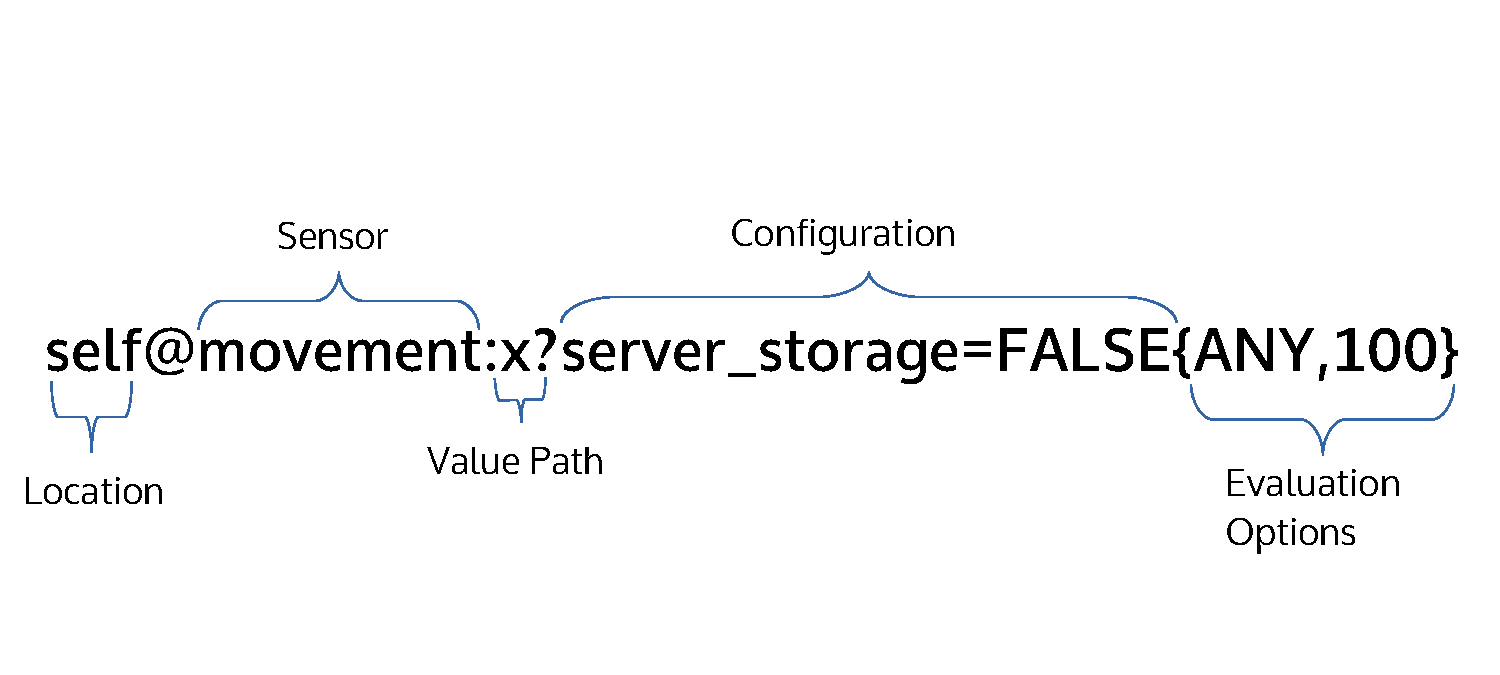
\includegraphics[scale=0.6]{Figures/swan_expr.pdf}
    \rule{35em}{0.5pt}
  \caption[Swan Expression]{Detailed swan expression).}
  \label{fig:SwanExpression}
\end{figure}

As part of our research we will also operate changes on the SWAN Song Expression and the meaning of different parameters.

\section{Beacon Frame Standards}
With Bluetooth Low Energy devices market in its incipient stage, the Beacon  emitters suffer from high fragmentation.
To help improve the situation, Apple and Google stepped up to offer frame specifications and further enforce the standard.

Apple's format, called iBeacon is simple and only focused on proximity applications.
On the other hand, Google offer and extensive standard, with 3 different frame specifications and more specifications coming soon.

%% Chapter Template

\chapter{SWAN Data Specifications} % Main chapter title

\label{Chapter4} % Change X to a consecutive number; for referencing this chapter elsewhere, use \ref{ChapterX}

\lhead{Chapter X. \emph{Chapter Title Here}} % Change X to a consecutive number; this is for the header on each page - perhaps a shortened title

%----------------------------------------------------------------------------------------
%	SECTION 1
%----------------------------------------------------------------------------------------

\section{Introduction}
Initially SWAN was designed to take a single value from the sensor data.
The value should be a primitive type such as Integer, Float, Double etc.
This constraint applies because SWAN evaluation engine allows the programmer to perform MIN, MAX and AVERAGE operations on given sensor data.
Also, History reduction is important when using the single value.

By adding multiple sensors, it became clear that taking a single value is not scalable enough. 
The further changes were delayed by adding multiple value paths to the sensor implementation. 
A clear example was accelerometer data: You will probably need the values for all 3 axis: x, y, z.
And you need to register 3 expressions for each value path.
The limitation can no longer be avoided after implementing Beacon Sensors, because now we need to add a full array of beacon identifiers under the same timestamp,
the key-value to provide individual temperature data or even key-array of values if we want the accelerometer data from all beacons.

%-----------------------------------
%	SUBSECTION 1
%-----------------------------------
\section{Proposed Solutions}
All the proposed solutions should met the following requirements:
\begin{itemize}
 \item Support multiple sensors of the same type(beacon sensor)
 \item Support multiple values for each sensor
 \item Provide scheme for single sensor single value data
 \item Provide implementation for Evaluation Engine Application
\end{itemize}

\subsection{Using a Mapping between keys and values to get all the data}
The format of data for the following function calls(value parameter):
\begin{lstlisting}[language=Java]
 AbstractSwanSensor.putValueTrimSize(final String valuePath,
					final String id,
					final long now,
					final Object value):
\end{lstlisting}

In order to satisfy the new requirements we propose the new data format to be encoded as: \begin{verbatim} Map<ValuePath, Map<sensorID,  ArrayList<Object>> \end{verbatim}

where:
\begin{itemize}
 \item ValuePath  = sensor valuepaths, ex Acceleromter x, y, z, total
 \item sensorID  =  self or unique Sensor Identifier(BeaconID)
\end{itemize}

We identify four sensor formats and recommend the following representation for each type of sensor:
\begin{itemize}
  \item Single Sensor Single Value(sensor name = stepcounter):
  \begin{itemize}
    \item \begin{verbatim} Example: Map: { steps={self=[13434545 ] }} \end{verbatim}                                                              
  \end{itemize}
 
  \item  Single Sensor, Multiple Values(sensor name =accelerometer):
  \begin{itemize}
    \item Key - name of the sensor
    \item Array of values - multiple values in the same order
    \item \begin{verbatim} Example: Map: { x={self=[0.5]},
                 y={self=[0.6]}, z={self=[-0.5]} } \end{verbatim}  
  \end{itemize}

 
  \item Multiple Sensor, Single Value(Beacon Distance):
  \begin{itemize}
    \item Key - the sensor identifier(id)
    \item Array of values - single value in the array
    \item  \begin{verbatim}  Example: Map: {distance={beaconID1=[1.5],
                 beaconID2=[0.5], beaconID3=[0.2]}} \end{verbatim}  
  \end{itemize}

  \item  Multiple Sensor, Multiple Values(sensor name = Beacon Accelerometer):
  \begin{itemize}
    \item Key - the sensor identifier(id), should be unique
    \item Array of values - multiple values in the same order
    \item  \begin{verbatim}  Example: Map:{x ={beaconID1=[-0.5], beaconID2=[-0.1],
                y = {beaconID1=[ 0.2], beaconID2=[-0.4]}} \end{verbatim}  
 \end{itemize}


\end{itemize}




%-----------------------------------
%	SUBSECTION 2
%-----------------------------------

\subsection{Subsection 2}

%----------------------------------------------------------------------------------------
%	SECTION 2
%----------------------------------------------------------------------------------------

\section{Implemented Approach}
 
%% Chapter Template

\chapter{Implementation Details} % Main chapter title

\label{Chapter5} % Change X to a consecutive number; for referencing this chapter elsewhere, use \ref{ChapterX}

\lhead{Chapter 5. \emph{Implementation Details}} % Change X to a consecutive number; this is for the header on each page - perhaps a shortened title

%----------------------------------------------------------------------------------------
%	SECTION 1
%----------------------------------------------------------------------------------------

\section{Swan Application Layout}
In the process of implementing the support for SWAN WEAR and Beacon Based Sensor, SWAN application layout has changed dramatically.

We will cover the following main changes operated to SWAN project structure during the last 6 months:
\begin{itemize}
 \item Splitting the SWAN project sources in libraries
 \item Uploading the SWAN JARS in publicly available repository - JCenter
\end{itemize}

Before each change change from above were made,  a merge of all SWAN repositories was made. You can read more about it in \hyperref[AppendixB]{Appendix B}.
Big changes on the project structure have a big impact on SWAN and could bring unexpected bugs.


\subsection{Splitting SWAN sources into libraries}\label{scc:swan_split}
After the implementation of the smartwatch sensors and beacon sensors, as part of research topic, SWAN had to be ported on smartwatch.
There were multiple options of how I was supposed to handle the challenge:
\begin{itemize}
 \item Clone all SWAN code and adapt it for the smartwatch
 \item Extract all common code and make it a library
\end{itemize}

I choose the second option, since it will avoid duplicate code and will allow easier maintenance in the future. As a starting point, I decided to see if The Evaluation Engine
code can be extracted and called from a library. The dependencies were extensive. The Evaluation Engine was depending on:
\begin{itemize}
 \item Swan Interface code - Classes that applications need to communicate with SWAN
 \item Swan Song Implementation - Parser and Data structure implementation for SWAN Expression
 \item Sensor Interfaces - used to implement new sensors in SWAN
 \item Beacon Implementation
 \item Proximity Implementation (SWAN Plus)
\end{itemize}

The first three components were separated from the SWAN Phone application and added to the swan core. Unfortunately, the dependency on the last two items
was still present and it had to be removed from the code, since the implementation was relevant only for phone and not for the smartwatch.
To preserve the functionality, all the methods depending on Proximity Manager and Beacon Discovery were replaced with empty bodies and the Evaluation Engine on
the phone was sub-classing the Evaluation Engine in the library and implementing the missing functionality.
The same design was applied to Abstract SWAN Sensor who was relying on Sense Android Library to offload values\cite{swan_layer}.

After \textbf{Swan Core} was made independent, we decided to extract \textbf{Swan Song} and \textbf{Swan Interface} from it and make them separate libraries.
The main reason for this library separation was the way applications interact with SWAN. Swan Interface are often imported as a separate jar in any application that want to register a 
SWAN expression. To improve the distribution of the Swan Interface, we decided to make it available on Android Main Repository - JCenter\cite{jcenter}. Uploading the Jars required us to follow the tutorial by The Cheese Factory\cite{jcenter_tutorial}.

Because we are maintaining the packages on JCenter now, the old packages and package building scripts  in the repository were discarded.
The JCenter  is not storing the packages in JAR format, but in the new format made to accommodate the Android Resources: AAR \cite{aar_format}. 
The new package format can be built and uploaded directly from Android Studio. Also, when changes are being operated on Swan Interface, 
the library versions should be updated accordingly:

\begin{itemize}
 \item If any change or addition  in the library was made, increment the patch version number: 1.0.0 $\rightarrow$1.0.1
 \item If any public class or Enumeration was deleted, increment the minor version: 1.0.0 $\rightarrow$ 1.1.0 
 \item The major version should be only incremented with SWAN major version: 1.0.0 $\rightarrow$ 2.0.0
\end{itemize}

More information about how to manage and upload swan libraries is available on SWAN wiki on Github\cite{swanWiki}

\section{Beacon based Bluetooth Sensors}

Bluetooth sensors allow us to get proximity data from the nearby beacons. Beacon sensor integration into SWAN expression based approach was not seamless.
The new data specifications which include beacon extension are discussed in \hyperref[Chapter3]{Chapter 3}.

Before exploring the implementation details we must discuss the available Beacon technology and Beacon Frame format.
The Bluetooth Low Energy Beacons can broadcast various data with different transmission power and broadcast interval.
The broadcast power is measured in dBm\cite{dbiRef}. The transmission power can vary from -30dBm and +4dBm. Higher transmit power
increase the range, but also shorten the battery life. The broadcast interval can vary from 300ms to more than 5 seconds. Higher resolution improves the accuracy of data,
especially for real-time applications, but also shorten the battery life.

To avoid the fragmentation of the Beacon Market, Google and Apple stepped in and proposed two standards for Beacon Frame Layout:
\begin{itemize}
 \item Apple iBeacon - simple beacon format, mostly used for proximity(distance measuring) applications
 \item Google Eddystone - complex standard, with 3 available frame formats:
 \begin{itemize}
  \item Eddystone UID - similar to iBeacon, broadcast unique ID
  \item EddystoneTLM - telemetry frame format, stores information about the beacon, such as temperature, battery level, number of packets sent
  \item Eddystone URL - frame layout which encodes a 17 bytes long URL in the frame
 \end{itemize}
\end{itemize}

The standards from above are industry recognized and widely implemented by various Beacon Manufacturers.
Unfortunately, even the Google Eddystone Format is not flexible enough and some companies need to come up with their own format to support extra functionality 
added to  their beacon products. We will also discuss the following frame formats which are proprietary to companies selling the test beacons, but they enable us to explore the
new way of using beacons:
\begin{itemize}
 \item AltBeacon Beacon Format - default beacon format present in the library used by SWAN for beacon scanning
 \item Estimote Nearable - Beacon Frame Format developed by Estimote\cite{estimote_company}, with accelerometer and movement data embedded into the format
\end{itemize}

The beacon implementation is revolving around adding support for the four beacon formats listed above. Implementation details were further split into 
following steps:
\begin{itemize}
 \item Implement Bluetooth Low Energy Scan
 \item Add support for existing Beacon Formats
 \item Implement Bluetooth Beacon Discovery
 \item Implement Bluetooth Based Sensors
\end{itemize}

\subsection{AltBeacon Library}
The AltBeacon Library is developed by Radius Networks\cite{radius_networks} company and provide a free and open-source implementation for applications that want to scan for beacons.
We choose to use this library over a custom implementation because of the easy way to add new beacon format. The library does not support beacons with encrypted 
identifiers, but it allows us to parse almost any existing, non-encrypting beacon frame. A proof of flexibility is our beacon layout for Estimote Nearable that we were able to 
implement in SWAN.
AltBeacon runs as a service, so SWAN needs to register to get the results of every scan. All the data from available beacons are available at once, so we decided to go for observer 
pattern, and register all sensors that want to access beacon data in our singleton class. This allows us to scan once for all sensors.

\subsection{Beacon Frame Formats}
The support for Apple iBeacon, Eddystone UID, Eddystone TLM, Eddystone URL and AltBeacon Format was already available in the library.
The Estimote format was left for us to analyse and provide the proper parsing expression to the AltBeacon Library.

The process of parsing the non- standard frame starts with finding the specifications for each byte in the frame. Fortunately, we found a NodeJs implementation 
who parses the Estimote Nearable Frame. The data encoded is presented in \hyperref[fig:estimote_format]{Figure 5.1}.
Before decoding the data we must tell the AltBeacon Library where to look for the frame identifier. The debugging mode allows us to see how the Bluetooth Low Energy frames are being parsed.

\subsection{Retrieving data from specific Beacons}
Original SWAN only allowed to return a single value of the primitive type. To comply with the new SWAN Data Specifications, we test the location part of expression to see which information we should provide:

\begin{itemize}
 \item If location is \textbf{self} we retrieve a random beacon from the list, which matches our frame type and give the result to the user
 \item if location contains a \textbf{beacon ID} we search for the beacon in list and if it is present, we will output the result
\end{itemize}

Other types of operations can be implemented, but first, a new revision of data formats should be made, to set the guidelines for all sensor implementations.

Our implementation relies on a singleton class which gets the result of the scanning and then distributes it to all registered beacon sensors. The AltBeacon library will automatically stop scanning
if no beacon sensors are registered.

\begin{figure}[htbp]
  \centering
    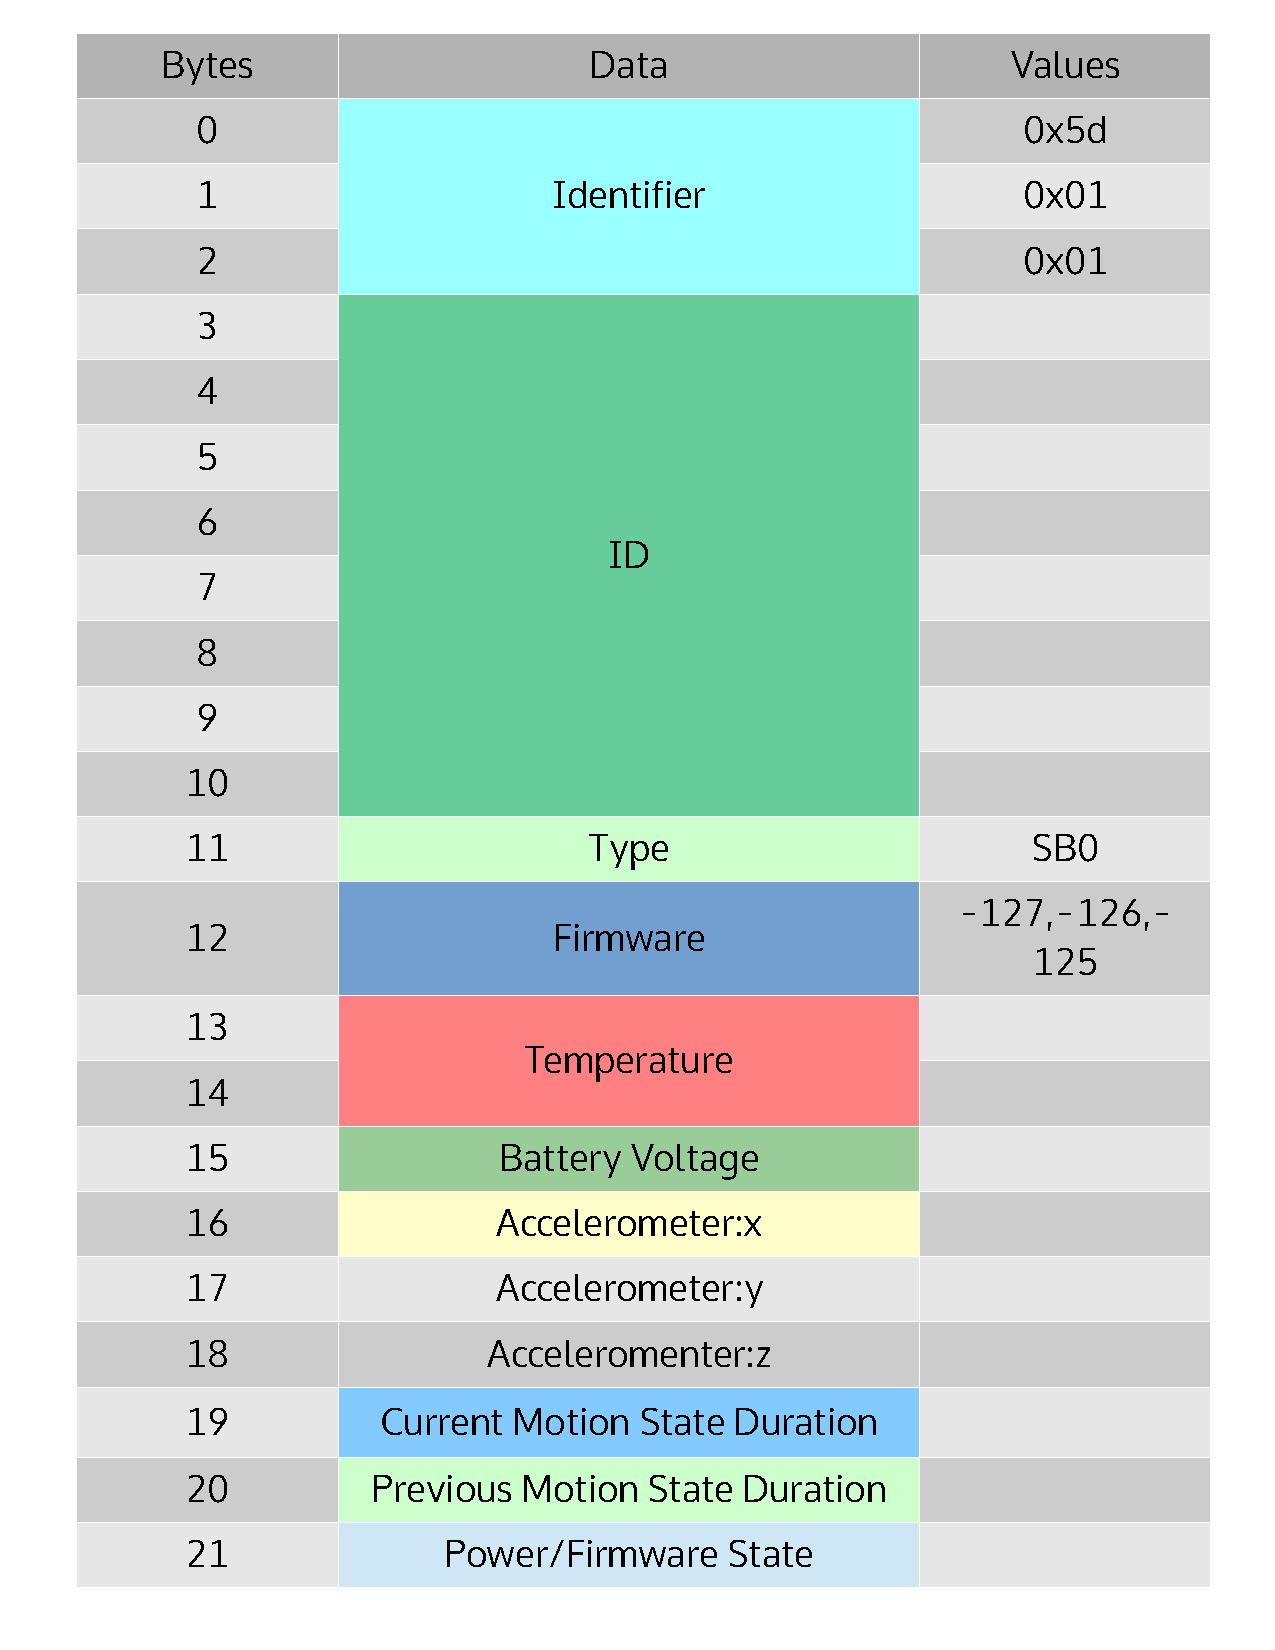
\includegraphics[scale=0.4]{Figures/data_format.pdf}
    \rule{35em}{0.5pt}
  \caption[Estimote Nearable Format]{Estimote Nearable Format}
  \label{fig:estimote_format}
\end{figure}

\section{ Value Based Smartwatch Sensors }
Implementing the value based smartwatch sensor was the first option and it derived from the Android's guidelines of performing the minimum amount of computation on the watch.
The other requirement was to keep code for Android Wear as small as possible, since the performance of the integrated components is lower compared to computing power on the smartphone.

To keep the implementation simple, we have a singleton class  responsible for communication between the smartphone and watch. We also issue start and stop commands to our service on the smartwatch,
so when no smartwatch sensor is active, the SWAN will not run on the watch.

We used the data path \cite{android_wear_datapath} for reliable communication between devices. The use of data path guarantee that the value will always be delivered at the cost of increased delay
and jitter\cite{jitter_ref} which affect our delay enforcing policy in SWAN.

The watch service is implemented as a foreground service\cite{foreground_service}. Running in foreground requires us to display the notification on the watch, but on the other hand we have the 
guarantee that our service will not be put to sleep by the operating system. 
Each SWAN sensor on the phone  is able to send start and stop commands, and the watch service will always count how many sensors are active. When no sensors are active, the service will stop.

Despite the Google's guidelines of keeping the Android Wear applications small, value based smartwatch sensors have poor energy efficiency. More about the power consumption experiment, 
in \hyperref[Chapter6]{Chapter 6}.

\section{Expression  Based  Smartwatch Sensors }

Expression based smartwatch sensor implementation aims to bring SWAN on your smartwatch. Before, we didn't consider to have SWAN on the watch a good idea. SWAN is a big application and running
it on the watch could result in sever performance issues on the watch. The opportunity on running SWAN on watch arisen after we managed to split SWAN source-code into \hyperref[scc:swan_split]{multiple libraries}. Some performance incurring features, such as database storage were left behind, and now the source-code was small enough to run on watch.

Compared to normal SWAN expression, a wear expression has the \hyperref[fig:SwanExpression]{location string} set to \textbf{wear} keyword. Evaluation Engine is responsible for changing the location
to \textbf{self} and forwarding the expression to SWAN on smartwatch.
The implementation of expression based smartwatch sensors added on top of the existing value based implementation. New commands were added to start and stop a swan expression on the watch.
The values sent back use the same implementation as for value based sensors. 

The main difference between value based and expression based sensors is that the values are not sent to SWAN sensor implementation for evaluation, but rather added to Evaluation Engine list of cached
values. This approach offers very low power consumption on the phone, as we can see from the power analysis in \hyperref[Chapter6]{Chapter 6}.
 
%% Chapter Template

\chapter{Power Efficiency Analysis} % Main chapter title

\label{Chapter6} % Change X to a consecutive number; for referencing this chapter elsewhere, use \ref{ChapterX}

\lhead{Chapter 6. \emph{Power Efficiency Analysis}} % Change X to a consecutive number; this is for the header on each page - perhaps a shortened title

%----------------------------------------------------------------------------------------
%	SECTION 1
%----------------------------------------------------------------------------------------

\section{Introduction}
The current implementation of the SWAN WEAR allows us to choose which way we want to process the data from the smartwatch application:
\begin{itemize}
 \item Perform minimum amount of computation on the watch and just send values to be processed by the SWAN PHONE application
 \item Send the expression to SWAN WEAR application for evaluation
\end{itemize}

Typically the recommended approach is to minimize the computation on the watch to save battery, but in certain cases,  when expression does not require frequent evaluation, we might get better power savings if we choose to perform the evaluation on the watch.

\section{Design}
Before proceeding to the data analysis, according to the GQM[4] paradigm, we should define the goal, the questions and the metrics.
    Our goal is to \textbf{analyze the power consumption} of phone and smartwatch, for the purpose of \textbf{comparing two different methods of acquiring sensor data}
    with respect to \textbf{differences in power consumption of phone and smartwatch}, in context of \textbf{SWAN android application}.

\textbf{Question 1}: What is the overhead of gaining data from smartwatch, compared to running evaluation on the watch?
\begin{itemize}
  \item Metric 1:  Battery level on Android Phone
  \item Metric 2:  Battery level on Android Smartwatch
  \item Metric 2:  Battery level on Android Smartwatch
  \item  Metric 3:  Expression runtime in seconds
\end{itemize}

\textbf{Question 2}:  What is the overhead of gaining data from test sensor compared to real hardware sensor?
\begin{itemize}
 \item Metric 1:  Battery level on Android Phone
 \item Metric 2: Battery level on Android Smartwatch
\end{itemize}

\section{Experiment Planning}
\subsection{Context Selection}
The experiment will be run on the simulated environment, composed of Android Phone and Android Wear Smartwatch. We will consider our experiment a real life problem because:
\begin{itemize}
 \item The tests are performed on real devices, which are used as reference for many android developers
 \item The test suite is composed of various sensor data, which reflect the actual SWAN performance in real life applications.
\end{itemize}

\subsection{Variable Selection}

The main dependent variable is \textbf{power consumption} expressed as battery power consumed after the experiment.
The independent variables are \textbf{data acquisition method} and \textbf{delay}.
Data acquisition method  have two options:
\begin{itemize}
 \item Phone based SWAN expressions
 \item Wear Based SWAN Expressions
\end{itemize}

Delay is set by us, but to avoid spending too much time on experiment, we will choose between two options: fast(100ms) and slow(1 second).

\subsection{ Hypothesis Formulation}

    We consider $\mu$ the battery power consumed by the test suite
    
    \textbf{Question 1:} What is the overhead of gathering data from smartwatch, compared to running evaluation on the watch? \newline
Conjecture(P): There is a difference between gaining data and evaluating expression on the smartwatch is significant \newline
Consequence(Q): The difference between only gaining data and evaluating expression on the smartwatch. \newline
\textit{Null hypothesis} - No observable difference in power consumption between only gathering data and evaluating expression on the watch \newline
H0 : ( $\mu$\textsubscript{phone} - $\mu$\textsubscript{wear} = 0) \newline
  Alternative hypothesis - There is a difference in power consumption between only gaining data on watch and running a SWAN expression on the watch \newline
H1:($\mu$\textsubscript{phone} - $\mu$\textsubscript{wear} $\neq$ 0)  \newline

    \textbf{Question 2:}  What is the overhead of gaining data from test sensor compared to real hardware sensor?\newline
    Conjecture(P): There is  a difference between using test sensor and real sensor on the smartwatch is significant\newline
    Consequence(Q): The difference between only gaining data and evaluating expression on the smartwatch is significant.\newline
    \textit{Null hypothesis} - No observable difference in power consumption between using test sensor and hardware sensor on the watch\newline
H0 : ($\mu$\textsubscript{test} - $\mu$\textsubscript{real} = 0)\newline
    Alternative hypothesis - There is a difference in power consumption between using test sensor and hardware sensor on the watch\newline
H1:($\mu$\textsubscript{test} - $\mu$\textsubscript{real} $\neq$ 0)\newline

\subsection{Subject Selection}
For this experiment we will use a batch of expressions targeting multiple sensors available on the smartwatch.
The batch for phone based tests contains the following expressions:
\begin{itemize}
 \item \begin{verbatim}self@wear_movement:x?delay={$delay}$server_storage=FALSE{ANY,0}\end{verbatim}
 \item \begin{verbatim}self@wear_gamerotation:x?delay={$delay}$server_storage=FALSE{ANY,0}\end{verbatim}
 \item \begin{verbatim}self@wear_linearacceleration:x?delay={$delay}$server_storage=FALSE{ANY,0}\end{verbatim}
 \item \begin{verbatim}self@wear_gravity:x?delay={$delay}$server_storage=FALSE{ANY,0}\end{verbatim}
 \item \begin{verbatim}self@wear_heartrate:heart_rate?delay={$delay}$server_storage=FALSE{ANY,0}\end{verbatim}
\end{itemize}

The batch for wear based expressions contains the following expressions:
\begin{itemize}
 \item \begin{verbatim}wear@movement:x?delay={$delay}$server_storage=FALSE{ANY,0}\end{verbatim}
 \item \begin{verbatim}wear@gamerotation:x?delay={$delay}$server_storage=FALSE{ANY,0}\end{verbatim}
 \item \begin{verbatim}wear@linearacceleration:x?delay={$delay}$server_storage=FALSE{ANY,0}\end{verbatim}
 \item \begin{verbatim}wear@gravity:x?delay={$delay}$server_storage=FALSE{ANY,0}\end{verbatim}
 \item \begin{verbatim}wear@heartrate:heart_rate?delay={$delay}$server_storage=FALSE{ANY,0}\end{verbatim}
\end{itemize}

The \textbf{\{\$delay\}} will be replaced by appropriate value when registering an expression

To evaluate the performance of the real sensor compared to test sensor, we will run the test sensor for the same 
amount of values and we will compare its power consumption with power consumption from hardware sensors. 
There will be 2 implementations of the test sensor, one for each data acquisition approach.

\subsection{Experiment Design}
For the first part of the experiment we will have two factors to vary: \textbf{data acquisition approach} and \textbf{delay}.
This will give us four different scenarios to test:

\begin{center}
  \begin{tabular}{ |l|l|l|l| }
  \hline
  \multicolumn{4}{ |c| }{Factor A: Data acquisition Method} \\
  \hline
  \multicolumn{2}{|c|}{Phone Based Evaluation}  & \multicolumn{2} {|c|}{Wear Based Evaluation} \\
  \hline
  \multicolumn{2}{|c|}{Factor B: Delay}  & \multicolumn{2} {|c|}{Factor B: Delay} \\
  \hline
  Delay: 100ms & Delay: 1000 ms & Delay: 100ms & Delay: 1000 ms\\
  \hline
  3x Experiments & 3x Experiments & 3x Experiments &3x Experiments\\
  \hline
  \end{tabular}
\end{center}

The second part of the experiment will focus on quantifying the discrepancy between power consumption when using a test sensor
versus using a real, hardware sensor.In this test scenario we also apply delay of 100 ms and 1000ms, to be fully aware of the implications of all factors.

\begin{center}
 \textbf{Delay 100 ms:}
\end{center}

\begin{center}
  \begin{tabular}{ |l|l|l|l| }
  \hline
  \multicolumn{4}{ |c| }{Factor A: Data acquisition Method} \\
  \hline
  \multicolumn{2}{|c|}{Phone Based Evaluation}  & \multicolumn{2} {|c|}{Wear Based Evaluation} \\
  \hline
  \multicolumn{2}{|c|}{Factor B: Sensor Type}  & \multicolumn{2} {|c|}{Factor B: Sensor Type} \\
  \hline
  Real Sensor & Test Sensor & Real Sensor & Test Sensor\\
  \hline
  3x Experiments & 3x Experiments & 3x Experiments &3x Experiments\\
  \hline
  \end{tabular}
\end{center}

\begin{center}
 \textbf{Delay 1000 ms:}
\end{center}

\begin{center}
  \begin{tabular}{ |l|l|l|l| }
  \hline
  \multicolumn{4}{ |c| }{Factor A: Data acquisition Method} \\
  \hline
  \multicolumn{2}{|c|}{Phone Based Evaluation}  & \multicolumn{2} {|c|}{Wear Based Evaluation} \\
  \hline
  \multicolumn{2}{|c|}{Factor B: Sensor Type}  & \multicolumn{2} {|c|}{Factor B: Sensor Type} \\
  \hline
  Real Sensor & Test Sensor & Real Sensor & Test Sensor\\
  \hline
  3x Experiments & 3x Experiments & 3x Experiments &3x Experiments\\
  \hline
  \end{tabular}
\end{center}

\subsection{Threats to Validity}
External: The experiment is being performed on specific setup. Even if the devices in our tests are chosen to represent the reference,
the android market is fragmented, and different android versions, hardware and smartwatches can yield to a different result

Internal: Basing our power consumption  results on battery levels increase the total error rate. Non linear discharge rate,
battery wear[5] can influence the final conclusion. To avoid these battery limitations, we will perform tests only when the battery is fully charged, 
so the discharge pattern will be the same. Also to reduce the battery wear impact, the tests will be performed with limited time delay,
and without any phone or smartwatch usage between the tests.

 Internal: The batch execution of the expression can induce extra error if different types of sensors have different power consumption. 
 We will try to limit the impact of this error type by proving that the selection of the sensors have the same power draw by
 performing single sensor benchmark with initial full battery. 
 
 Internal: The communication using Bluetooth may vary energy consumption based on distance or obstacles between devices.
 We minimize the impact of Bluetooth, by placing phone and smartwatch in close proximity with no obstacles in between.
 
 External: Heart rate sensor can be unpredictable. In some circumstances, the heart rate sensor can stop giving values. 
 Since we were not wearing the watching during our test, were placed it on the charging dock, with no charging cable connected and the phone
 in close proximity. By satisfying this conditions, the experiment setup and results can be verified.
 
 \subsection{Instrumentation}
 The following devices are available to perform our experiment:
 \begin{itemize}
  \item Phone - Nexus 6P - manufactured by Huaweii,  with latest Android 6.0 Marshmallow installed and with Android security patch level: 1 June 2016. 
  \item Smartwatch - Motorola 360 gen 2, with latest Android 6.0 Marshmallow, android wear version 1.5 
 \end{itemize}

 We could have a bigger selection of phones to run SWAN on them, since we only have one smartwatch available,
 the different processors  and Bluetooth chips might induce more random in our observations.
 Besides we can argue that Nexus phones are used by default by a lot smartwatch manufacturers for tests.
 Before proceeding to experiment setup, the devices were factory reset and the only android wear app necessary for smartwatch connection was installed.
 We observed that by default a lot of Google applications are installed on the Nexus Phone. Some of them also have watch apps packaged.
 To avoid possible battery drain from other applications we decided to disable the following apps on the Nexus Phone:
 \begin{itemize}
  \item  Google Drive
  \item Google Play Games
  \item Google Play Music
  \item Hangouts
  \item Google Maps
  \item Google Photos
  \item Youtube
  \item Google Docs
 \end{itemize}

 Measuring power consumption of both approaches require us to have accurate tools for measuring power consumption.
 The power consumption should be measured on both phone and android wear device, so we could better understand what are the pros and cons of using each method.
 We have two methods of measuring the power consumption:
 \begin{itemize}
  \item Using the android battery starts, which provide the current power draw if the device is equipped with a hardware fuel gauge(Our test devices Nexus 6P and Moto 360 gen 2 )[1]
  \item The standard setup: Running each method for a prolonged amount of time and measure the battery level after the experiment is done
 \end{itemize}

 Using the hardware power gauge is a very useful feature to measure the power consumption. Unfortunately it suffers from two major disadvantages:
 \begin{itemize}
  \item We require to run another battery sensor, so the results may not reflect the constant power consumption of the swan application running
  \item Hardware fuel gauge has it's own limitations, and the computed power usage may not be accurate
 \end{itemize}

 Using battery level measurement can also be affected by battery maximum capacity, charge-discharge cycle, but since we repeat the experiment for both options on the same hardware, and without delay we can argue that results can be compared.
 Additionally, measuring the battery levels allow us to have a better average value.
 
 \subsection{Experiment Execution}
 After initial research we concluded that the data from hardware fuel gauge is highly inaccurate on Android Wear.
 The reason is exceptionally power efficient hardware and high error rate for power consumption sensor. 
 Also we are unable to test what is the power implication of running the SWAN WEAR foreground service. 
 In order to obtain some power metrics, we will monitor battery levels on phone and smartwatch after SWAN expression returns a given amount of sensor values, in both scenarios.
The results that we might will be analyzed based on power consumption on both phone and smartwatch.
The experiment steps should be performed in the following order:
\begin{itemize}
 \item Factory reset both phone and smartwatch.
 \item Pair smartwatch to the phone
 \item Install swan on the phone and smartwatch
 \item Run a preliminary test, to see if swan is ready to operate
 \item Charge both phone and smartwatch to 100%
 \item Install test application
 \item Disable Wi-Fi and radio, leave only Bluetooth
 \item Start test application and turn off the screen of the phone
 \item Test application should take the phone and wear battery levels and remaining Power values before starting test evaluations
 \item Wait for application to finish the test suite
 \item Test application will take the battery levels and remaining power values after the tests are finished and will write them on local storage for further analysis
\end{itemize}

For the testing purpose, we will avoid sensors that are dependent of user motion to actually work: 
\begin{itemize}
 \item Step counter sensor - will send updates only if the user walked after last query. It might also be related to hardware implementation of the sensor in our test device. 
 \item Light sensor - the updates are triggered by changes in light level and since our test setup is configured to run for a long time, we can not include a sensor triggered by external,
 undefined behaviour
\end{itemize}

Surprisingly, the Heart Rate Sensor will still give you values even if it is not mounted on the wrist, so we can use it for our test purpose. 
Heart rate sensor is different compared to regular sensors found on the phone. The smallest granularity for heart rate results is one second,
so specifying a smaller delay will not make any sense.  Delays bigger than one second instead will fulfilled by SWAN implementation.
 
 \subsection{Preliminary Tests}
Preliminary tests shows us that we can not rely on the estimated power reported by the fuel gauge sensors. In case of our phone device,
Nexus 6P, the reported values in nano-watts were not accurate at all. Instead, the current discharge current was reported, 
but we can not use it in our tests, since it will interfere with our test setup.
We encountered the similar problem on our smartwatch, Motorola 360 generation 2. 
The reported value in nano-Watts was not corresponding with the maximum theoretical energy that the watch battery is able to hold, according to the specifications.
The current power consumption value.
On the other hand the formulas for running the specified amount of time are accurate, we recorded a deviation of +- 5% of run time for different types of sensors 

To get comparable results we are supposed to guarantee equal conditions for both test scenarios.
Since SWAN is quite power efficient and sensors that we are targeting are also very power efficient, the test should run for a long period of time.
We estimated that a notable difference in battery levels should occur after running SWAN expressions for around two hours period.
Running tests for longer period of time can help us identify even smaller differences, 
but the necessity of running the experiments with different type of expressions and also the number of repetitions for each scenario make the use of longer runtimes prohibitive.
Also we should take into consideration the charging time necessary after each run of the experiment,
with smartwatch normally loosing the biggest battery percentage  and having long recharge times.

\subsection{Test Application}
The test application was build in order to run tests in batch order and gather the battery level data. To avoid power consumption from external sources, such as phone screen, we implemented the testing code as foreground service[3] which is not hibernated by the android system when the screen is off. 
The testing application has the following workflow:
For each SWAN expression:
\begin{itemize}
 \item Register a swan expression and get the battery level of the phone before the experiment
 \item Register a swan expression and get the battery level of the smartwatch before the experiment
 \item Register the start time
 \item Calculate the number of values necessary for the run, based on the given expected runtime in microseconds
 \item Register the experiment expressions and wait until the number of values are reached
 \item Register expression end time
 \item Get the battery level of the phone after the experiment
 \item Get the battery level of the smartwatch after the experiment
\end{itemize}


Once the tests for expression is done, the application will write on local storage, in a text file the expressions name,
battery levels before and after for each device the number of values received and the total runtime.
 The values are comma separated, so it can be imported in Excel for further processing.

Even if the program runs in a separate service, we are not allowed to block in the main thread. 
We are actually required to wait for the SWAN expression to terminate, so we sent the computation in another thread and we used Latch to wait for expression execution.

 \section{Results}
 
%% Chapter Template

\chapter{Conclusion and Future Work} % Main chapter title

\label{Chapter7} % Change X to a consecutive number; for referencing this chapter elsewhere, use \ref{ChapterX}

\lhead{Chapter 7. \emph{Conclusion and Future Work}} % Change X to a consecutive number; this is for the header on each page - perhaps a shortened title

%----------------------------------------------------------------------------------------
%	SECTION 1
%----------------------------------------------------------------------------------------

\section{Conclusions}

%-----------------------------------
%	SUBSECTION 1
%-----------------------------------
\section{Future Work}
 

%----------------------------------------------------------------------------------------
%	THESIS CONTENT - APPENDICES
%----------------------------------------------------------------------------------------

\addtocontents{toc}{\vspace{2em}} % Add a gap in the Contents, for aesthetics

\appendix % Cue to tell LaTeX that the following 'chapters' are Appendices

% Include the appendices of the thesis as separate files from the Appendices folder
% Uncomment the lines as you write the Appendices

% Appendix A

\chapter{Appendix Title Here} % Main appendix title

\label{AppendixA} % For referencing this appendix elsewhere, use \ref{AppendixA}

\lhead{Appendix A. \emph{Appendix Title Here}} % This is for the header on each page - perhaps a shortened title

Write your Appendix content here.
%% Appendix Template

\chapter{Merging SWAN Repositories} % Main appendix title

\label{AppendixB} % Change X to a consecutive letter; for referencing this appendix elsewhere, use \ref{AppendixX}

\lhead{Appendix B. \emph{Merging SWAN Repositories}} % Change X to a consecutive letter; this is for the header on each page - perhaps a shortened title
At the beginning of the master thesis project, the main repository of SWAN was holding the stable version of it, which was being used in production 
by a  company. Our SWAN project has a big team, each member work on different part of the SWAN or SWAN related functionality.
To avoid any breaking changes to the current SWAN version, we decided to make a different branch and put all my smartwatch related changes in it.
When we was done with implementing the first prototype of SWAN WEAR sensors, other PhD students' projects: SWAN Plus\cite{swan_plus} and SWAN-Fly\cite{swan_fly} were also ready.
Unfortunately, the commits of the projects stated above were in different repositories so merging them into master branch was proven to be difficult.
We followed this procedure when merging the SWAN:
\begin{itemize}
 \item Create the release branch with the old, stable SWAN
 \item Create development branches for SWAN Plus and SWAN-Fly
 \item Export commits from SWAN Plus and SWAN-Fly as patches
 \item Apply the patches to each development branch
 \item Merge Smartwatch code into Master
 \item Merge SWAN Plus into master and resolve conflicts
 \item Merge SWAN-Fly into master and resolve conflicts
\end{itemize}

The most challenging part was to apply patches from the two different repositories. Merging commits were the reason why some history was 
lost, and patches were hard to apply. This also proves why you should always use the rebase option instead of merging option when you push commits
to the remote. Atlassian article\cite{atlassian_merge_rebase} explains the main advantage of rebasing over using merging commits.
%\input{Appendices/AppendixC}

\addtocontents{toc}{\vspace{2em}} % Add a gap in the Contents, for aesthetics

\backmatter

%----------------------------------------------------------------------------------------
%	BIBLIOGRAPHY
%----------------------------------------------------------------------------------------

\label{Bibliography}

\lhead{\emph{Bibliography}} % Change the page header to say "Bibliography"

\bibliographystyle{apalike} % Use the "apalike" BibTeX style for formatting the Bibliography

\bibliography{Bibliography} % The references (bibliography) information are stored in the file named "Bibliography.bib"

\end{document}